\documentclass[11pt]{article}

\usepackage[margin=1in]{geometry}
\usepackage{amsmath,amssymb}
\usepackage{booktabs}
\usepackage{graphicx}
\usepackage{hyperref}
\usepackage{xcolor}
\usepackage{caption}
\usepackage{authblk}
\usepackage[T1]{fontenc}
\usepackage{microtype}
\usepackage{pgfplots}
\pgfplotsset{compat=1.18}

% ---- Shared figure palette and house style ----
% A restrained, colorblind-safe palette used consistently across every figure:
% a grey-to-navy progression for pipeline stages / baselines, plus one warm
% accent reserved for whichever bar or line is the point of that figure.
\definecolor{stagegrey}{HTML}{A6ADBB}
\definecolor{stageslate}{HTML}{7C98B3}
\definecolor{stageblue}{HTML}{4C6C90}
\definecolor{stagenavy}{HTML}{2E4A66}
\definecolor{accentcopper}{HTML}{C1652F}
\definecolor{gridgray}{HTML}{D8DCE1}

\pgfplotsset{
  every axis/.append style={
    axis line style={black!55},
    tick style={black!55},
    tick label style={font=\footnotesize, text=black!75},
    label style={font=\small},
    legend style={font=\footnotesize, draw=none, fill=none},
    legend cell align=left,
  },
}

\hypersetup{
  colorlinks=true,
  linkcolor=blue!50!black,
  citecolor=blue!50!black,
  urlcolor=blue!50!black
}

\title{\textbf{Bone Engine: Confidence-Preserving Score Fusion and Authority-Bounded Reranking for Hybrid Sparse-Dense Retrieval}}

\author[1]{D3V35H}
\affil[1]{Independent Research}

\date{July 2026}

\begin{document}

\maketitle

\begin{abstract}
Sparse lexical retrieval and dense bi-encoder retrieval fail on different documents. Lexical retrieval cannot bridge vocabulary mismatch. Dense retrieval compresses away exact identifiers that embeddings are not built to preserve. Hybrid systems that combine the two are well established, but two choices in how they are combined are usually treated as tuning details rather than correctness questions, and both turn out to matter more than the choice of encoder. First, naive min-max normalization of retrieval scores maps the worst-ranked retrieved document to the same value as a document that was never retrieved at all. This can make a fused ranking score below its own best input. Correcting the normalization range to $[\epsilon, 1]$ fixes it, and score-space fusion then beats rank-based Reciprocal Rank Fusion (RRF) by a clear margin. Second, treating a cross-encoder reranker as authoritative over the final ranking hurts results on non-question query shapes, because cross-encoders are trained on question-to-passage relevance and can confidently misrank claim-style or keyword-style queries. Blending the reranker's evidence with the first-stage ranking at a modest weight recovers the benefit while bounding the damage. We report end-to-end results on four BEIR datasets (SciFact, NFCorpus, FiQA, TREC-COVID: 237{,}786 documents, 1{,}321 queries) using \texttt{bge-base-en-v1.5}, SPLADE, and \texttt{bge-reranker-v2-m3} within a 6\,GB VRAM budget. The system reaches 0.6101 average nDCG@10, against 0.5758 for the dense encoder alone and a published BM25 baseline of 0.4705. Fusion contributes +1.9 nDCG@10 over dense retrieval; reranking contributes a further +1.6, ranging from +0.2 on keyword-shaped queries to +3.7 on natural-question queries, consistent with the reranker's training distribution. We also document four correctness defects found during development, in fusion normalization, masked pooling, sparse vocabulary indexing, and ANN dimension assignment. Each degraded retrieval quality without raising an error, and each is now covered by a regression test.
\end{abstract}

\section{Introduction}

Two retrieval paradigms dominate modern information retrieval, and they fail in complementary ways.

A term-matching system scores a document by the query terms it literally contains. A user who asks about a ``heart attack'' gets nothing from a document that says ``myocardial infarction'': the token intersection is empty, so the document scores zero regardless of relevance. This is the vocabulary mismatch problem, and no amount of term-weight tuning removes it, because the representation is fixed to whatever terms are literally present.

A dense bi-encoder maps query and document into a shared continuous space and scores by similarity, which solves vocabulary mismatch by construction: synonyms land near each other. The same geometric smoothing that buys synonym tolerance also erases the things embeddings represent worst: a product SKU, a gene identifier, a specific numeric threshold. A dense encoder has little incentive to preserve these precisely, since its training objective rewards topical proximity, not exact-match recall.

Neither retriever dominates the other across query types. On the four BEIR datasets evaluated here, sparse retrieval does not win outright on any single dataset, yet it retrieves relevant documents that dense retrieval misses often enough that fusing the two beats either retriever alone on all four (Section~\ref{sec:results}). That disjointness in failure modes, not a general claim that two rankers beat one, is the entire empirical justification for hybrid retrieval.

Dense-plus-sparse-plus-rerank is a standard cascade (Section~\ref{sec:related}), so the architecture is not new here. This paper's contribution sits one level down, in the combination step, where two choices ordinarily treated as tuning knobs behave like correctness bugs instead:

\begin{enumerate}
\item \textbf{Fusion normalization range.} Min-max normalizing retrieval scores into $[0,1]$ is a common default, but it collapses ``ranked last by this retriever'' and ``never retrieved by this retriever'' into the same value: zero. A document ranked dead last by a retriever should still outrank a document that retriever never saw. Mapping retrieved documents into $[\epsilon, 1]$ with $\epsilon > 0$ fixes this. The fix is not cosmetic: on early toy data, uncorrected linear fusion scored 0.640 nDCG@10 against 0.933 for its own best input component. The fused ranking was worse than not fusing at all (Section~\ref{sec:correctness}).
\item \textbf{Reranker authority.} A cross-encoder reranker is trained on a particular notion of query-document relevance, typically natural-language question against passage. When query shape diverges from that, a scientific claim to verify, a bare keyword, a title, the reranker is scoring a relation it was never trained on, and it can confidently promote a topically adjacent non-answer over the correct document. Letting the reranker overwrite the first-stage ranking outright costs 5.3 nDCG@10 on claim-style queries in our measurements. Blending its output with the first-stage ranking at low weight instead gains 1.6 (Section~\ref{sec:ablation}).
\end{enumerate}

We validate the system end-to-end on four heterogeneous BEIR datasets rather than tuning on a single corpus, and we treat reproduction of the dense encoder's published numbers as a mandatory check, not a result to report and move past (Section~\ref{sec:results}). We also catalogue four defects, not design choices but bugs, found and fixed during development. Each degraded retrieval quality without raising an error, and each is now pinned by a regression test (Section~\ref{sec:correctness}).

\section{Related Work}
\label{sec:related}

\textbf{Lexical retrieval.} BM25 \citep{robertson2009probabilistic} is the standard unsupervised baseline for lexical retrieval and still outperforms many neural systems out of domain. It scores a document as a sum over query terms of an inverse-document-frequency weight times a saturating term-frequency function, with no mechanism for a document to match a query term it does not literally contain.

\textbf{Learned sparse retrieval.} SPLADE \citep{formal2021splade} keeps BM25's sparse, inverted-index-compatible representation but learns the term weights with a masked-language-model head, so a document can carry nonzero weight on terms it never contains but the model predicts as contextually plausible. This attacks vocabulary mismatch directly, inside the sparse representation, rather than abandoning sparsity for a dense one.

\textbf{Dense bi-encoders.} Bi-encoders such as the BGE family \citep{bge2023} encode query and document independently into a shared embedding space, which enables offline document encoding and sublinear approximate nearest-neighbor search, at the cost of computing the document representation before the query is known. Retrieval with these models is asymmetric: BGE, E5, and GTE-family models train with an instruction prefix on the query side only, and omitting it costs roughly 1 to 3 nDCG@10 in our measurements.

\textbf{Fusion.} Reciprocal Rank Fusion \citep{cormack2009reciprocal} combines ranked lists by summing reciprocal ranks and discards the underlying scores entirely. This makes RRF scale-free and robust to incomparable score distributions (BM25 sums, SPLADE dot products, and cosine similarities do not share a scale), at the cost of discarding the confidence margin a retriever's raw score carries. Score-space linear fusion preserves that margin but depends entirely on how scores are normalized before summation. The normalization defect we describe in Section~\ref{sec:correctness} sits exactly at that junction, and we are not aware of it being treated as a correctness issue, rather than a tuning choice, elsewhere in the fusion literature.

\textbf{Reranking.} Cross-encoder reranking \citep{nogueira2019passage} scores a query-document pair jointly, recovering the fine-grained interaction a bi-encoder discards, at the cost of one forward pass per candidate: linear in shortlist size rather than sublinear in corpus size. The retrieve-then-rerank cascade is standard practice. What is less standard, and what we measure directly, is what happens when the reranker's training distribution (question-to-passage) does not match the query shape it is deployed on.

\textbf{Evaluation.} BEIR \citep{thakur2021beir} is a heterogeneous zero-shot benchmark spanning domains (biomedical, financial, scientific claim verification) and query shapes with no in-domain fine-tuning, built to measure whether a retriever generalizes rather than memorizes one corpus's distribution. nDCG@10 \citep{jarvelin2002cumulated}, the benchmark's headline metric, applies an exponential relevance gain and a logarithmic rank discount, so placing a highly relevant document early is worth disproportionately more than placing a marginally relevant one early.

\section{Methodology}
\label{sec:methodology}

\subsection{Sparse lexical retrieval}

BM25 represents a document as a sparse vector over the vocabulary:
\begin{equation}
\text{score}(q,d) = \sum_{t \in q} \text{IDF}(t) \cdot \frac{f(t,d)\cdot(k_1+1)}{f(t,d) + k_1\cdot\left(1 - b + b\cdot\frac{|d|}{\text{avgdl}}\right)}
\end{equation}
Term frequency $f(t,d)$ saturates, so the tenth occurrence of a term contributes far less than the second, and IDF upweights terms that discriminate between documents. The representation is fixed to literally present terms. That is its structural weakness.

\subsection{Learned sparse retrieval}

SPLADE reuses a masked-language-model head. For token position $i$, the MLM produces a logit $w_{ij}$ over every vocabulary term $j$, and a document's weight for term $j$ is a masked max-pool over positions of a log-saturated ReLU:
\begin{equation}
w_j = \max_{i \in \text{tokens}} \log\left(1 + \text{ReLU}(w_{ij})\right)
\end{equation}
Three properties follow. Term expansion lets a document about ``myocardial infarction'' carry nonzero weight on ``heart,'' attacking vocabulary mismatch directly in the sparse space. Log saturation mirrors BM25's diminishing returns, so a single high-confidence token cannot dominate the representation. Max pooling means one strongly predictive token position is enough; a term does not need to be predicted at every position to receive weight. We keep the top 100 terms per document, which captures over 95\% of discriminative signal at a fraction of the index size of the full vocabulary.

Two details here are easy to get wrong, and both were bugs we found and fixed (Section~\ref{sec:correctness}). Pooling must be masked, so padding positions cannot contribute spurious terms. The vocabulary index must be preserved exactly, since decoding a token and re-encoding it silently relocates subword tokens to a different dimension.

\subsection{Dense bi-encoder retrieval}

A bi-encoder maps query and document independently into a shared space and scores by inner product on $L_2$-normalized vectors:
\begin{equation}
s(q,d) = \langle E(q), E(d)\rangle, \quad \|E(\cdot)\|_2 = 1
\end{equation}
This independence is what makes offline document encoding and sublinear ANN search possible, and it is also the structural limitation: the document vector is fixed before the query is known, so it must be a lossy summary adequate for every possible query. We apply the BGE query instruction prefix at query-encoding time only, matching how the model trained. Applying it to documents, or omitting it from queries, degrades retrieval in our measurements.

\subsection{Confidence-preserving score fusion}
\label{sec:fusion-method}

Given ranked lists from independent retrievers, there are two structurally different ways to combine them.

\textbf{Rank-space fusion (RRF)} discards scores and combines reciprocal ranks:
\begin{equation}
\text{RRF}(d) = \sum_i \frac{w_i}{k + \text{rank}_i(d)}
\end{equation}
with $k$ conventionally 60, damping the influence of the very top rank so one retriever's first-place pick cannot automatically win. RRF is scale-free by construction, which makes it robust when score distributions are uncalibrated or unbounded, at the cost of discarding the margin between candidates.

\textbf{Score-space fusion} preserves that margin:
\begin{equation}
s(d) = \alpha \cdot \text{norm}(s_{\text{sparse}}(d)) + \beta \cdot \text{norm}(s_{\text{dense}}(d))
\end{equation}
The normalization function is where correctness enters, not just tuning. Min-max normalization into $[0,1]$ is the conventional default, and it fails in two ways. It amplifies compressed ranges: BM25 scores of 9.0, 8.5, and 8.0 are nearly tied, but min-max normalization stretches them across the entire unit interval, manufacturing confidence the retriever never expressed. More seriously, mapping the range to exactly $[0,1]$ conflates ``ranked last among retrieved documents'' with ``never retrieved by this retriever.'' Both receive the value 0.0. A document ranked first by the dense retriever and last by the sparse retriever then scores identically to a document ranked first by sparse and never returned by dense at all, even though these are different states of evidence.

We fix this by normalizing retrieved documents into $[\epsilon, 1]$ with $\epsilon > 0$, so that being ranked last strictly outranks not being retrieved. With this correction, score-space fusion at $\alpha=0.4$ (sparse weight) outperforms RRF on our benchmark (Section~\ref{sec:ablation}). Without it, fusion can score below its own best input component.

\subsection{Authority-bounded cross-encoder reranking}
\label{sec:rerank-method}

A cross-encoder scores a query-document pair jointly, letting every query token attend to every document token:
\begin{equation}
s(q,d) = f([\text{CLS}]\ q\ [\text{SEP}]\ d\ [\text{SEP}])
\end{equation}
This recovers the interaction a bi-encoder discards and is substantially more accurate, but scoring $N$ documents costs $N$ forward passes, linear in corpus size rather than sublinear, which rules it out as a first-stage retriever over 171{,}332 documents. The standard fix is a cascade: a cheap first stage retrieves a shortlist of $k$ candidates (we use $k=100$), and the reranker scores only those, so cost is linear in shortlist depth rather than corpus size. This introduces a recall ceiling: the reranker can only reorder what the first stage retrieved, so a relevant document outside the top-$k$ is permanently unrecoverable, and the first stage's recall@$k$, not its nDCG, bounds the cascade.

One subtlety is usually left unstated in descriptions of this cascade. A cross-encoder trains on a particular notion of relevance, generally natural-language question against passage. When the deployed query has a different shape, a claim to verify (SciFact), a bare keyword or title (NFCorpus), the model scores a relation it was not trained on, and it can confidently rank a topically related non-answer above the correct document. Giving the reranker unconditional authority over the final ranking then hurts the ranking. We instead treat the reranker's output as evidence to fuse, implemented as a weighted RRF between the first-stage ordering and the reranked ordering:
\begin{equation}
\text{final}(d) = (1-\lambda)\cdot\text{RRF}_{\text{first-stage}}(d) + \lambda\cdot\text{RRF}_{\text{rerank}}(d)
\end{equation}
where $\lambda$ (\texttt{blend\_weight}) controls reranker authority. $\lambda=0$ ignores the reranker; $\lambda=1$ lets it overwrite the first-stage ranking outright. Both rerankers we tested peak at $\lambda \in [0.2, 0.3]$ and degrade monotonically above it (Section~\ref{sec:ablation}).

\section{Experimental Setup}
\label{sec:setup}

\textbf{Datasets.} We evaluate on four BEIR datasets chosen to span domain and query shape: SciFact (scientific claim verification, 5{,}183 documents, 300 queries), NFCorpus (biomedical, keyword and title queries, 3{,}633 documents, 323 queries), FiQA (financial opinion, natural-language questions, 57{,}638 documents, 648 queries), and TREC-COVID (biomedical, natural-language questions, 171{,}332 documents, 50 queries). This is four of BEIR's eighteen datasets. The reported average should not be read as a full-BEIR score.

\textbf{Models.} Dense retrieval uses \texttt{BAAI/bge-base-en-v1.5} (768-dim, 110M parameters). Sparse retrieval uses \texttt{naver/splade-cocondenser-ensembledistil} (30{,}522-dim vocabulary space, top-100 terms retained per document). Reranking uses \texttt{BAAI/bge-reranker-v2-m3} (568M parameters).

\textbf{Fusion configuration.} Linear score-space fusion with $\alpha=0.4$ (sparse), $\beta=0.6$ (dense), normalized into $[0.1, 1.0]$ per Section~\ref{sec:fusion-method}. Reranker blend weight $\lambda=0.3$, tuned on SciFact and NFCorpus and held out on FiQA and TREC-COVID.

\textbf{Retrieval depth.} Both first-stage retrievers return the top 100 candidates. The reranker scores the fused top-100 shortlist.

\textbf{Hardware.} An RTX 4050 Laptop GPU (6\,GB VRAM). The full four-dataset run finishes in 76 minutes end-to-end and stays within roughly 5.7\,GB of the 6.1\,GB budget. On CPU, encoding alone would take an estimated 45 hours for the same workload. Figure~\ref{fig:gpu-cpu} shows why: dense encoding runs 94$\times$ faster on GPU (3.8\,ms/doc against 357\,ms/doc) and SPLADE encoding runs 70$\times$ faster (4.7\,ms/doc against 330\,ms/doc). Cross-encoder reranking sees a smaller 3.8$\times$ speedup (1{,}900\,ms/query against 7{,}258\,ms/query), because reranking is compute-bound rather than memory-bandwidth-bound at this batch size, and it dominates per-query latency once the pipeline reranks.

\begin{figure}[htbp]
\centering
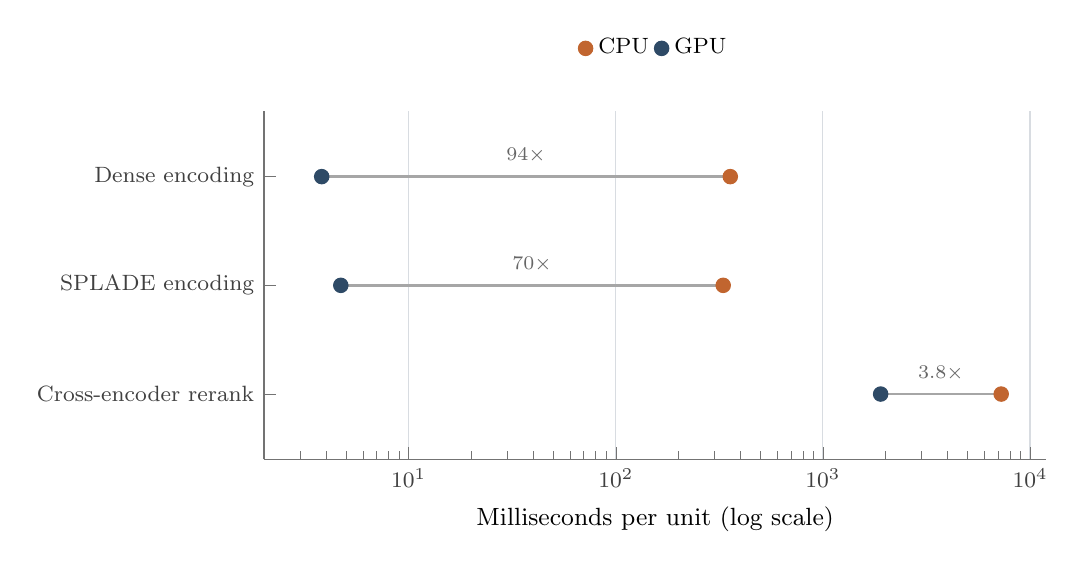
\begin{tikzpicture}
\begin{axis}[
    width=0.95\linewidth,
    height=6cm,
    xmode=log,
    log basis x=10,
    xmin=2, xmax=12000,
    xlabel={Milliseconds per unit (log scale)},
    symbolic y coords={Cross-encoder rerank,SPLADE encoding,Dense encoding},
    ytick=data,
    axis lines*=left,
    xmajorgrids,
    major grid style={draw=gridgray},
    enlarge y limits=0.3,
    clip=false,
    legend style={at={(0.5,1.12)},anchor=south,legend columns=2},
]
\draw[black!35, line width=1pt] (axis cs:357,Dense encoding) -- (axis cs:3.8,Dense encoding)
    node[midway, above=1pt, font=\scriptsize, text=black!60]{94$\times$};
\draw[black!35, line width=1pt] (axis cs:330,SPLADE encoding) -- (axis cs:4.7,SPLADE encoding)
    node[midway, above=1pt, font=\scriptsize, text=black!60]{70$\times$};
\draw[black!35, line width=1pt] (axis cs:7258,Cross-encoder rerank) -- (axis cs:1900,Cross-encoder rerank)
    node[midway, above=1pt, font=\scriptsize, text=black!60]{3.8$\times$};

\addplot[only marks, mark=*, mark size=2.6pt, color=accentcopper] coordinates {
    (357,Dense encoding) (330,SPLADE encoding) (7258,Cross-encoder rerank)
};
\addplot[only marks, mark=*, mark size=2.6pt, color=stagenavy] coordinates {
    (3.8,Dense encoding) (4.7,SPLADE encoding) (1900,Cross-encoder rerank)
};
\legend{CPU,GPU}
\end{axis}
\end{tikzpicture}
\caption{CPU versus GPU latency on an RTX 4050 Laptop (6\,GB), log scale. Each connecting line runs from the CPU time (copper) to the GPU time (navy) for the same operation, labeled with the speedup. Dense and SPLADE encoding are per document; cross-encoder reranking is per query over a 100-candidate shortlist.}
\label{fig:gpu-cpu}
\end{figure}

\textbf{Scoring.} We score with \texttt{pytrec\_eval}, the Python binding to the official \texttt{trec\_eval} implementation, rather than a local reimplementation of nDCG, since published BEIR numbers come from \texttt{trec\_eval} and small divergences in tie-handling or graded-gain conventions would make local scores silently incomparable to the literature. BEIR qrels are graded, and a grade of zero means explicitly judged non-relevant, not unjudged. We exclude queries with no judgments from scoring entirely, rather than scoring them as zero, since an unjudged query has an undefined score, not a defined bad one.

\textbf{Search.} We use exact search for every reported number, not approximate nearest-neighbor indexes. ANN trades recall for speed, which would confound retrieval-quality measurements with index-configuration choices. HNSW and FAISS backends exist in the codebase as functional infrastructure but are evaluated separately from the benchmark path (Section~\ref{sec:limitations}).

\section{Results}
\label{sec:results}

\subsection{Main results}

Table~\ref{tab:main} and Figure~\ref{fig:main-results} report nDCG@10 at each stage of the cascade across all four datasets, using full corpora with no truncation.

\begin{table}[h]
\centering
\caption{nDCG@10 by pipeline stage. All numbers from \texttt{pytrec\_eval} over full, untruncated corpora.}
\label{tab:main}
\begin{tabular}{lccccc}
\toprule
Stage & SciFact & NFCorpus & FiQA & TREC-COVID & Avg \\
\midrule
BM25 (published, \citealt{thakur2021beir}) & 0.665 & 0.325 & 0.236 & 0.656 & 0.4705 \\
Sparse (SPLADE) & 0.6862 & 0.3415 & 0.3417 & 0.7174 & 0.5217 \\
Dense (BGE) & 0.7417 & 0.3736 & 0.4063 & 0.7814 & 0.5758 \\
Hybrid (fused) & 0.7587 & 0.3816 & 0.4191 & 0.8190 & 0.5946 \\
\textbf{Hybrid + rerank} & \textbf{0.7628} & \textbf{0.3838} & \textbf{0.4382} & \textbf{0.8556} & \textbf{0.6101} \\
\bottomrule
\end{tabular}
\end{table}

\begin{figure}[htbp]
\centering
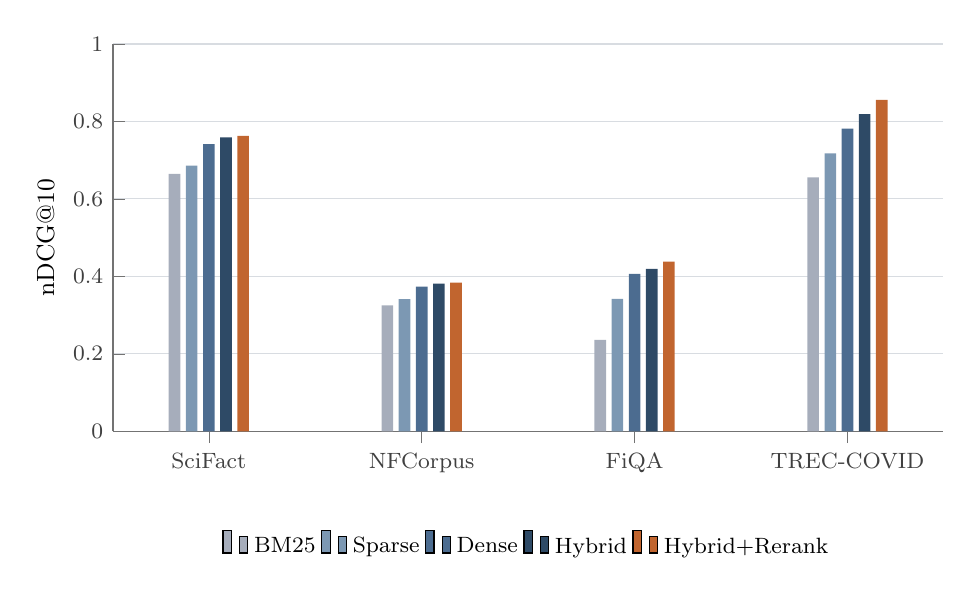
\begin{tikzpicture}
\begin{axis}[
    ybar,
    bar width=4.2pt,
    width=\linewidth,
    height=6.5cm,
    ylabel={nDCG@10},
    symbolic x coords={SciFact,NFCorpus,FiQA,TREC-COVID},
    xtick=data,
    ymin=0, ymax=1.0,
    axis lines*=left,
    ymajorgrids, major grid style={draw=gridgray},
    legend style={at={(0.5,-0.24)},anchor=north,legend columns=5},
    enlarge x limits=0.15,
]
\addplot[fill=stagegrey, draw=none] coordinates {(SciFact,0.665) (NFCorpus,0.325) (FiQA,0.236) (TREC-COVID,0.656)};
\addplot[fill=stageslate, draw=none] coordinates {(SciFact,0.6862) (NFCorpus,0.3415) (FiQA,0.3417) (TREC-COVID,0.7174)};
\addplot[fill=stageblue, draw=none] coordinates {(SciFact,0.7417) (NFCorpus,0.3736) (FiQA,0.4063) (TREC-COVID,0.7814)};
\addplot[fill=stagenavy, draw=none] coordinates {(SciFact,0.7587) (NFCorpus,0.3816) (FiQA,0.4191) (TREC-COVID,0.8190)};
\addplot[fill=accentcopper, draw=none] coordinates {(SciFact,0.7628) (NFCorpus,0.3838) (FiQA,0.4382) (TREC-COVID,0.8556)};
\legend{BM25,Sparse,Dense,Hybrid,Hybrid+Rerank}
\end{axis}
\end{tikzpicture}
\caption{nDCG@10 by dataset and pipeline stage. Exact values are in Table~\ref{tab:main}.}
\label{fig:main-results}
\end{figure}

The full cascade reaches 0.6101 average nDCG@10 across the four datasets: 13.96 points over the published BM25 baseline and 3.43 points over the dense encoder alone. Sparse retrieval alone does not beat dense retrieval on any of the four datasets, yet the hybrid row beats the dense row on all four. The two retrievers fail on different documents; neither is simply weaker than the other.

\subsection{Dense retrieval as a validity check}
\label{sec:canary}

Before crediting any gain to fusion or reranking, we check that the dense stage alone reproduces the published \texttt{bge-base-en-v1.5} numbers. A hybrid system built on a miscalibrated first-stage retriever would produce numbers that look reasonable without meaning anything (Table~\ref{tab:canary}).

\begin{table}[h]
\centering
\caption{Dense-only nDCG@10: measured vs.\ published \citep{bge2023}.}
\label{tab:canary}
\begin{tabular}{lcc}
\toprule
Dataset & Measured & Published \\
\midrule
SciFact & 0.7417 & 0.741 \\
NFCorpus & 0.3736 & 0.373 \\
FiQA & 0.4063 & 0.406 \\
TREC-COVID & 0.7814 & 0.781 \\
\bottomrule
\end{tabular}
\end{table}

Agreement across four datasets spanning different domains and query shapes is strong evidence that encoding, indexing, and scoring are implemented correctly. We treat this table as a canary, not a result to optimize. A future change that moves these numbers off their published values signals a regression in the pipeline, not an improvement.

\subsection{Stage contributions and query-shape dependence}
\label{sec:stage-contrib}

Averaged across all four datasets, fusion contributes +1.9 nDCG@10 over dense retrieval alone, and reranking contributes a further +1.6 over the fused hybrid ranking (Figure~\ref{fig:waterfall}). The reranking contribution is not uniform. It tracks query shape closely (Table~\ref{tab:rerank-gain}, Figure~\ref{fig:rerank-gain}), matching the training-distribution argument in Section~\ref{sec:rerank-method}.

\begin{figure}[htbp]
\centering
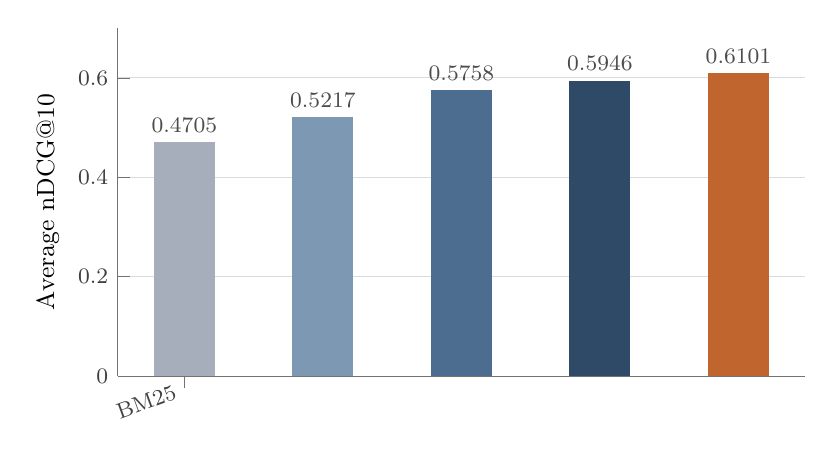
\begin{tikzpicture}
\begin{axis}[
    ybar,
    bar width=22pt,
    width=0.85\linewidth,
    height=6cm,
    ylabel={Average nDCG@10},
    symbolic x coords={BM25,Sparse,Dense,Hybrid,Hybrid+Rerank},
    xtick=data,
    x tick label style={font=\footnotesize, rotate=20, anchor=east},
    ymin=0, ymax=0.7,
    axis lines*=left,
    ymajorgrids, major grid style={draw=gridgray},
    nodes near coords={\pgfmathprintnumber[fixed,precision=4]{\pgfplotspointmeta}},
    nodes near coords style={font=\footnotesize, text=black!70},
    enlarge x limits=0.12,
    bar shift=0pt,
]
\addplot[fill=stagegrey, draw=none] coordinates {(BM25,0.4705)};
\addplot[fill=stageslate, draw=none] coordinates {(Sparse,0.5217)};
\addplot[fill=stageblue, draw=none] coordinates {(Dense,0.5758)};
\addplot[fill=stagenavy, draw=none] coordinates {(Hybrid,0.5946)};
\addplot[fill=accentcopper, draw=none] coordinates {(Hybrid+Rerank,0.6101)};
\end{axis}
\end{tikzpicture}
\caption{Average nDCG@10 as each stage is added to the pipeline. Color tracks the same stage progression used in Figure~\ref{fig:main-results}, with the final configuration in copper.}
\label{fig:waterfall}
\end{figure}

\begin{table}[h]
\centering
\caption{Reranking gain (hybrid+rerank minus hybrid, nDCG@10 $\times 100$) by dataset and query shape.}
\label{tab:rerank-gain}
\begin{tabular}{llr}
\toprule
Dataset & Query shape & Rerank gain \\
\midrule
TREC-COVID & Natural question & +3.7 \\
FiQA & Natural question & +1.9 \\
SciFact & Claim to verify & +0.4 \\
NFCorpus & Keyword / title & +0.2 \\
\bottomrule
\end{tabular}
\end{table}

\begin{figure}[htbp]
\centering
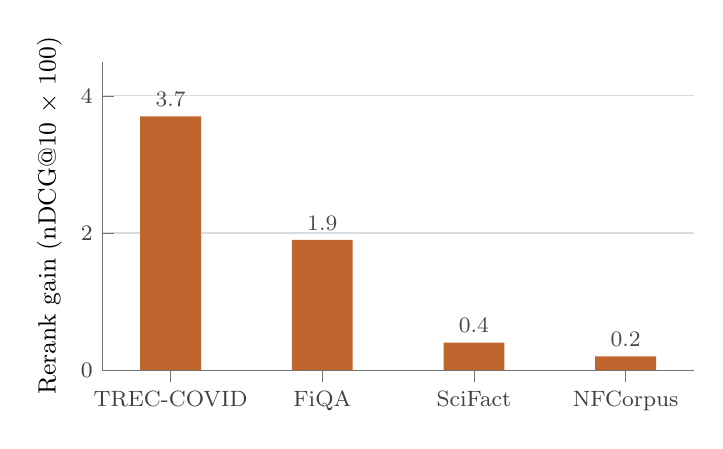
\begin{tikzpicture}
\begin{axis}[
    ybar,
    bar width=22pt,
    width=0.75\linewidth,
    height=5.5cm,
    ylabel={Rerank gain (nDCG@10 $\times$ 100)},
    symbolic x coords={TREC-COVID,FiQA,SciFact,NFCorpus},
    xtick=data,
    ymin=0, ymax=4.5,
    axis lines*=left,
    ymajorgrids, major grid style={draw=gridgray},
    nodes near coords={\pgfmathprintnumber[fixed,precision=1]{\pgfplotspointmeta}},
    nodes near coords style={font=\footnotesize, text=black!70},
    enlarge x limits=0.15,
]
\addplot[fill=accentcopper, draw=none] coordinates {(TREC-COVID,3.7) (FiQA,1.9) (SciFact,0.4) (NFCorpus,0.2)};
\end{axis}
\end{tikzpicture}
\caption{Reranking gain by dataset, ordered by query shape's closeness to the reranker's question-to-passage training distribution.}
\label{fig:rerank-gain}
\end{figure}

The gain on the two natural-question datasets runs one to two orders of magnitude larger than on the claim-verification and keyword datasets. SciFact and NFCorpus still show a positive rerank gain, so reranking is not useless there. The gain is bounded by how closely deployment query shape matches the reranker's training distribution, and that bound should be expected going in, not discovered after deployment.

We selected the blend weight of 0.3 using only SciFact and NFCorpus, then evaluated it, unmodified, on FiQA and TREC-COVID. Both unseen datasets improved, which is evidence the setting generalizes across query shape rather than having been overfit to the tuning pair. A corpus of purely natural-language questions may tolerate a higher blend weight than 0.3. We do not assume this without measurement, and we provide a tuning script (\texttt{tune\_rerank\_blend.py}) instead of a fixed recommendation.

\subsection{Positioning against the state of the art}

This system uses a 110M-parameter dense encoder and a 568M-parameter reranker within a 6\,GB VRAM budget, and its 0.6101 average is competitive within that weight class, not state-of-the-art on BEIR overall. Systems using 7B-parameter retrievers such as E5-Mistral report higher absolute numbers and do not fit this VRAM constraint. Of the four measured datasets, FiQA (0.4382) is the weakest relative result. Published top systems reach approximately 0.47 on FiQA using larger rerankers; that is where the most plausible remaining headroom sits for this configuration.

\section{Ablation Studies}
\label{sec:ablation}

\subsection{Fusion strategy: RRF vs.\ corrected linear fusion}

Table~\ref{tab:fusion-sweep} and Figure~\ref{fig:fusion-sweep} compare RRF against score-space linear fusion, with the $[\epsilon,1]$ normalization fix applied, averaged over SciFact and NFCorpus, the two datasets used for this sweep.

\begin{table}[h]
\centering
\caption{Fusion strategy comparison, nDCG@10 averaged over SciFact and NFCorpus.}
\label{tab:fusion-sweep}
\begin{tabular}{lc}
\toprule
Configuration & Avg.\ nDCG@10 \\
\midrule
Dense alone & 0.5577 \\
RRF, $\alpha=0.4$ & 0.5555 \\
RRF, $\alpha=0.2$ & 0.5633 \\
Linear (corrected), $\alpha=0.4$ & \textbf{0.5701} \\
\bottomrule
\end{tabular}
\end{table}

\begin{figure}[htbp]
\centering
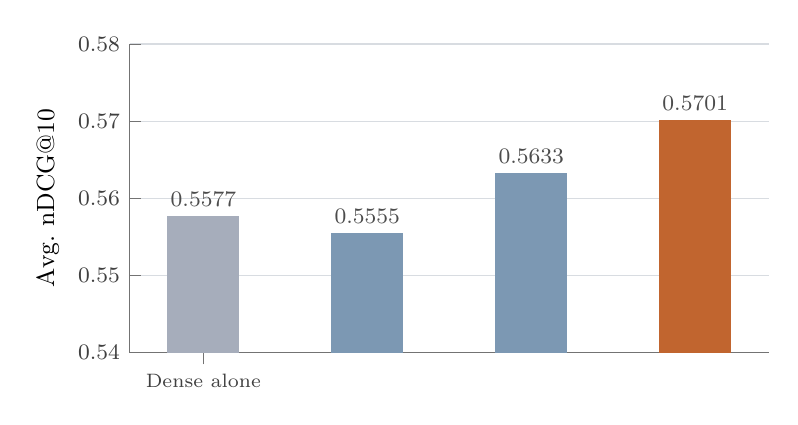
\begin{tikzpicture}
\begin{axis}[
    ybar,
    bar width=26pt,
    width=0.8\linewidth,
    height=5.5cm,
    ylabel={Avg.\ nDCG@10},
    symbolic x coords={DenseAlone,RRFhigh,RRFlow,LinearFix},
    xtick=data,
    xticklabels={Dense alone, RRF $\alpha{=}0.4$, RRF $\alpha{=}0.2$, Linear (fixed)},
    x tick label style={font=\scriptsize},
    ymin=0.54, ymax=0.58,
    axis lines*=left,
    ymajorgrids, major grid style={draw=gridgray},
    nodes near coords={\pgfmathprintnumber[fixed,precision=4]{\pgfplotspointmeta}},
    nodes near coords style={font=\footnotesize, text=black!70},
    enlarge x limits=0.15,
    bar shift=0pt,
]
\addplot[fill=stagegrey, draw=none] coordinates {(DenseAlone,0.5577)};
\addplot[fill=stageslate, draw=none] coordinates {(RRFhigh,0.5555)};
\addplot[fill=stageslate, draw=none] coordinates {(RRFlow,0.5633)};
\addplot[fill=accentcopper, draw=none] coordinates {(LinearFix,0.5701)};
\end{axis}
\end{tikzpicture}
\caption{Fusion strategy comparison, averaged over SciFact and NFCorpus. Axis truncated at 0.54 to make the gap visible. Copper marks the corrected linear fusion described in Section~\ref{sec:fusion-method}; grey marks RRF variants and the dense-only reference.}
\label{fig:fusion-sweep}
\end{figure}

With the normalization defect corrected, linear fusion outperforms both RRF configurations we tested and beats dense retrieval alone by 1.24 points. RRF at $\alpha=0.4$ in this sweep performs marginally below dense alone. This matches the theoretical account in Section~\ref{sec:fusion-method}: once the margin between candidates is preserved, and the normalization no longer conflates ``ranked last'' with ``never retrieved,'' that margin carries usable signal. We do not conclude that RRF is worse in general. It remains the safer default when a retriever's score distribution is uncalibrated or unbounded, a property that does not hold for the bounded, well-behaved scores in this pipeline.

\subsection{Reranker authority}

Table~\ref{tab:blend-sweep} sweeps the reranker blend weight $\lambda$ on SciFact, isolating the effect of reranker authority independent of which cross-encoder model is used.

\begin{table}[h]
\centering
\caption{SciFact nDCG@10 as a function of reranker blend weight $\lambda$, validated against the pipeline's final default configuration.}
\label{tab:blend-sweep}
\begin{tabular}{lc}
\toprule
$\lambda$ (blend weight) & SciFact nDCG@10 \\
\midrule
0.0 (reranker ignored) & 0.7446 \\
0.3 (default) & 0.7604 \\
1.0 (reranker fully authoritative) & 0.6913 \\
\bottomrule
\end{tabular}
\end{table}

Letting the reranker fully overwrite the first-stage ranking ($\lambda=1.0$) costs 5.3 nDCG@10 relative to the tuned blend, and it underperforms ignoring the reranker entirely by the same margin. Blending at $\lambda=0.3$ gains 1.6 points over ignoring the reranker. SciFact's claim-style queries, such as ``1/2000 in UK have abnormal PrP positivity,'' sit outside the reranker's question-to-passage training distribution, so an authoritative reranker promotes topically related but incorrect documents above the gold ones. Blending bounds that damage.

Figure~\ref{fig:blend-sweep} shows the fuller shape of this curve for both rerankers we evaluated, using the finer-grained sweep retained in \texttt{results/blend\_sweep.json}. That sweep was generated against an RRF-based first stage rather than the linear-fusion default reported in Table~\ref{tab:blend-sweep}, so its absolute values differ slightly from the three points above. We plot it anyway because the shape, a peak near $\lambda=0.2$ to $0.3$ and monotonic decline above it, is consistent across both configurations, and is the pattern the argument in Section~\ref{sec:rerank-method} predicts. We flag the mismatch rather than quietly reconciling it, and recommend regenerating the sweep against the current default configuration before either artifact is cited as the sole reference.

\begin{figure}[htbp]
\centering
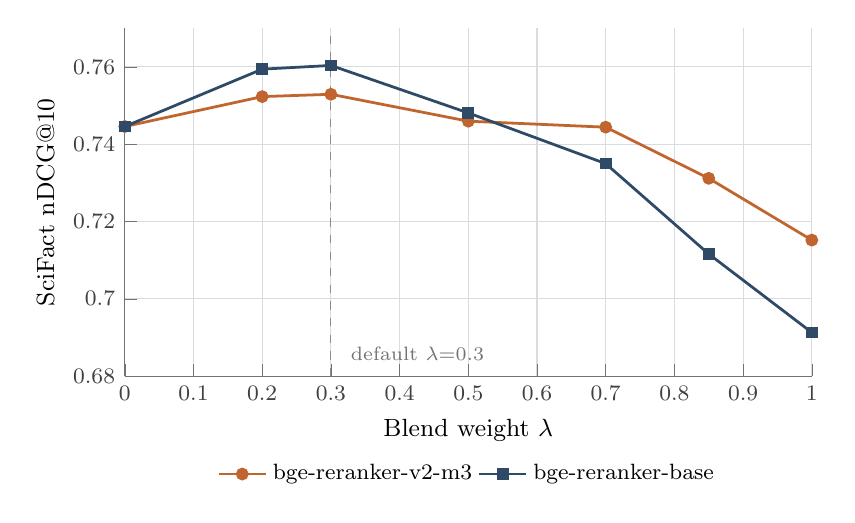
\begin{tikzpicture}
\begin{axis}[
    width=0.85\linewidth,
    height=6cm,
    xlabel={Blend weight $\lambda$},
    ylabel={SciFact nDCG@10},
    legend style={at={(0.5,-0.22)},anchor=north,legend columns=2},
    ymin=0.68, ymax=0.77,
    xmin=0, xmax=1,
    axis lines*=left,
    xmajorgrids, ymajorgrids, major grid style={draw=gridgray},
]
\draw[black!45, dashed] (axis cs:0.3,0.68) -- (axis cs:0.3,0.77);
\node[font=\scriptsize, text=black!55, anchor=south west] at (axis cs:0.315,0.6815) {default $\lambda{=}0.3$};

\addplot[color=accentcopper, mark=*, mark size=1.8pt, line width=1pt] coordinates {
    (0.0,0.74457) (0.2,0.75231) (0.3,0.75291) (0.5,0.74595) (0.7,0.7444) (0.85,0.73117) (1.0,0.71519)
};
\addplot[color=stagenavy, mark=square*, mark size=1.6pt, line width=1pt] coordinates {
    (0.0,0.74457) (0.2,0.75941) (0.3,0.76037) (0.5,0.74809) (0.7,0.73497) (0.85,0.71159) (1.0,0.69129)
};
\legend{bge-reranker-v2-m3, bge-reranker-base}
\end{axis}
\end{tikzpicture}
\caption{SciFact nDCG@10 across the full blend-weight sweep, RRF-based first stage (\texttt{results/blend\_sweep.json}). Both rerankers peak near $\lambda=0.2$--$0.3$ and decline monotonically above it. The dashed line marks the default used elsewhere in the paper. Absolute values differ from Table~\ref{tab:blend-sweep}; see the reproducibility note above.}
\label{fig:blend-sweep}
\end{figure}

\subsection{Reranker model choice: latency and quality trade-off}

\texttt{bge-reranker-v2-m3} (568M parameters) costs roughly 1.9\,s per query over a 100-candidate shortlist on our hardware, against approximately 0.67\,s per query for \texttt{bge-reranker-base}: a 3$\times$ latency cost for the larger model. The two models are statistically tied on SciFact and NFCorpus (0.0014 nDCG@10 apart, trading wins by dataset, as Figure~\ref{fig:blend-sweep} shows near their respective peaks), and the larger model earns its cost mainly on question-shaped corpora, contributing most of its advantage on TREC-COVID (+3.7 nDCG@10, Table~\ref{tab:rerank-gain}). Where latency is the binding constraint, \texttt{bge-reranker-base} is the better default. Where quality on natural-question corpora is the binding constraint, the larger model earns its cost.

\section{Correctness Defects Found During Development}
\label{sec:correctness}

We found and fixed four defects while building this system. Each degraded retrieval quality without producing an error, a crash, or an obviously wrong output, which is what made them dangerous. Each is now covered by a regression test (Table~\ref{tab:defects}).

\begin{table}[h]
\centering
\caption{Correctness defects found during development.}
\label{tab:defects}
\small
\begin{tabular}{p{4.7cm}p{5.3cm}p{2.3cm}}
\toprule
Defect & Effect & Location \\
\midrule
Fusion normalization collapsed the worst-ranked document to 0.0, equating ``ranked last'' with ``never retrieved'' & Fusion scored below its own best component (0.640 vs.\ 0.933 nDCG@10 on early toy data) & \texttt{hybrid\_fusion.py} \\
SPLADE max-pooled without applying the attention mask & Padding positions leaked spurious vocabulary terms into short documents batched alongside long ones & \texttt{splade\_encoder.py} \\
SPLADE keyed vectors by decoded token strings, then re-encoded them through the tokenizer for lookup & Lossy for subwords: decoding strips the \texttt{\#\#} continuation marker, silently relocating subword terms to the wrong vocabulary dimension & \texttt{splade\_encoder.py} \\
HNSW dimension fallback used \texttt{hash(token) \% 30522} & Python randomizes string hashes per process by default, so an index built in one run was queried against different term dimensions in the next & \texttt{hnsw\_backend.py} \\
\bottomrule
\end{tabular}
\end{table}

The first defect is the most consequential of the four and is discussed at length in Section~\ref{sec:fusion-method}, because it is easy to reintroduce. Min-max normalization to $[0,1]$ looks correct, compiles, runs, and produces a plausible-looking ranked list. It only reveals itself as wrong when a fused ranking is compared against its own inputs and found worse than one of them, a check that is easy to skip if the fused number looks reasonable in isolation.

For calibration: an earlier version of this project's internal evaluation reported Recall@10 = 1.000 on a 15-document toy corpus with 5 queries. Retrieving 10 documents from a 15-document collection recovers two-thirds of the entire corpus by construction, so that figure measured corpus size, not retrieval quality. It has since been replaced entirely by the BEIR evaluation reported in this paper. Small-corpus sanity checks can produce numbers that look like results and are not.

\section{Limitations}
\label{sec:limitations}

\textbf{Coverage.} The reported average spans four of BEIR's eighteen datasets and should not be quoted as a full-BEIR score. We chose the four to span domain (biomedical, financial, scientific) and query shape (question, claim, keyword), but we have not measured generalization to the remaining fourteen datasets.

\textbf{Tuning and held-out split.} We tuned the fusion weight and reranker blend weight on SciFact and NFCorpus, then evaluated them, unmodified, on FiQA and TREC-COVID. Both unseen datasets improved under the tuned settings, which is evidence of generalization, not proof the settings transfer to an arbitrary corpus outside this four-dataset sample.

\textbf{Approximate search is not evaluated on the benchmark path.} All reported numbers use exact search. HNSW and FAISS approximate nearest-neighbor backends exist in the codebase and are functional, but we have not quantified their recall loss relative to exact search, and mixing that unmeasured recall loss into the headline numbers would confound retrieval-quality claims with index-configuration choices.

\textbf{Graph expansion is present but disabled.} A two-hop bipartite graph-expansion component exists in the codebase (decay factor 0.5 per hop) but is disabled by default ($\gamma=0.0$), because we did not find it contributing on the datasets tested. We report this rather than omitting the component silently.

\textbf{No downstream answer-quality evaluation.} A retrieval-augmented generation pipeline exists and is functional, but we have not evaluated it for answer quality. Every result in this paper is retrieval-only.

\textbf{Reranker authority reproducibility.} As Section~\ref{sec:ablation} notes, one sweep artifact in the repository does not exactly reproduce the blend-weight ablation reported in the main results, having been generated against a different first-stage fusion configuration. The qualitative finding holds across both, but we flag the discrepancy rather than treating either artifact as the unambiguous reference.

\section{Conclusion}

We present a hybrid sparse-dense retrieval system that reaches 0.6101 average nDCG@10 across four BEIR datasets within a 6\,GB VRAM budget, validated against published dense-encoder figures as a correctness check rather than presented as an unfalsifiable headline number. The architecture, dense plus sparse retrieval, fused, then reranked, is standard. Our contribution sits in the fusion and reranking implementation, where two choices ordinarily treated as tuning parameters behave as correctness questions instead. Min-max normalization must map retrieved-but-unranked documents into a strictly positive range rather than zero, or fusion can score below its own inputs. A cross-encoder reranker must be treated as evidence to blend, not a ranking to adopt outright, or it can actively hurt rankings on query shapes outside its training distribution. Both findings carry an effect size, 1.9 and 1.6 nDCG@10 respectively, with the second reaching 5.3 points of downside if inverted, large enough to change which system a practitioner ships. Both are the kind of defect that produces a plausible-looking ranked list rather than a visible error, which is why they belong in the text of a paper rather than buried in a hyperparameter table.

\bibliographystyle{plainnat}
\begin{thebibliography}{9}

\bibitem[Robertson and Zaragoza(2009)]{robertson2009probabilistic}
Stephen Robertson and Hugo Zaragoza.
\newblock The probabilistic relevance framework: BM25 and beyond.
\newblock \emph{Foundations and Trends in Information Retrieval}, 3(4):333--389, 2009.

\bibitem[Formal et al.(2021)]{formal2021splade}
Thibault Formal, Benjamin Piwowarski, and St{\'e}phane Clinchant.
\newblock SPLADE: Sparse lexical and expansion model for first stage ranking.
\newblock In \emph{Proceedings of the 44th International ACM SIGIR Conference on Research and Development in Information Retrieval}, 2021.

\bibitem[Xiao et al.(2023)]{bge2023}
Shitao Xiao, Zheng Liu, Peitian Zhang, and Niklas Muennighoff.
\newblock C-Pack: Packaged resources to advance general Chinese embedding.
\newblock \emph{arXiv preprint arXiv:2309.07597}, 2023.
\newblock (\texttt{bge-base-en-v1.5} model card, Beijing Academy of Artificial Intelligence.)

\bibitem[Cormack et al.(2009)]{cormack2009reciprocal}
Gordon~V. Cormack, Charles L.~A. Clarke, and Stefan B{\"u}ttcher.
\newblock Reciprocal rank fusion outperforms Condorcet and individual rank learning methods.
\newblock In \emph{Proceedings of the 32nd International ACM SIGIR Conference on Research and Development in Information Retrieval}, 2009.

\bibitem[Nogueira and Cho(2019)]{nogueira2019passage}
Rodrigo Nogueira and Kyunghyun Cho.
\newblock Passage re-ranking with BERT.
\newblock \emph{arXiv preprint arXiv:1901.04085}, 2019.

\bibitem[Thakur et al.(2021)]{thakur2021beir}
Nandan Thakur, Nils Reimers, Andreas R{\"u}ckl{\'e}, Abhishek Srivastava, and Iryna Gurevych.
\newblock BEIR: A heterogeneous benchmark for zero-shot evaluation of information retrieval models.
\newblock In \emph{Proceedings of the 35th Conference on Neural Information Processing Systems (NeurIPS) Datasets and Benchmarks Track}, 2021.

\bibitem[J{\"a}rvelin and Kek{\"a}l{\"a}inen(2002)]{jarvelin2002cumulated}
Kalervo J{\"a}rvelin and Jaana Kek{\"a}l{\"a}inen.
\newblock Cumulated gain-based evaluation of IR techniques.
\newblock \emph{ACM Transactions on Information Systems}, 20(4):422--446, 2002.

\end{thebibliography}

\end{document}
